
\chapter{Litt om referering til rapportelementer}\label{kap:referering}

\section{{\em Tagging} av rapportelement, \fbox{\tt $\backslash$label\{ \}}}\label{delkap:label}
For at du i teksten du skriver 
skal kunne referere til forskjellige rapportelementer må du legge til en
{\em tag} eller {\em bookmark} som tydelige identifiserer selve
elementet. Til dette bruker du kommandoen 
\fbox{\tt $\backslash$label\{ \} }, hvor det som står inne i
krøllparentesene er den unike referanseteksten/identifikasjonen for elementet.
Siden det finnes veldig mange forskjellige rapportelementer som det kan
refereres til, er det vanlig å bygge opp selve referanseteksten slik:\\[-10mm]
\begin{center}
  {\tt $\backslash$label\{forkortelse for elementet:\underline{beskrivende tekst}\}}
\end{center}
\vspace*{-5mm}
Eksempler på typiske rapportelementer og forkortelser  er
vist i listen under, hvor {\tt xxxxx} er satt inn for \underline{\tt
  beskrivende tekst}.
\vspace*{-3mm}
\begin{enumerate}
\item For å referere til {\color{red}kapitler} benyttes ofte \fbox{\tt kap} som
  forkortelse\footnote{Dersom du vil bruke engelske ord er \fbox{\tt
      ch}  for {\tt $\backslash$chapter} et godt alternativ.}, og  
  {\tt $\backslash$label\{kap:xxxxx\}} må plasserers innenfor selve
  kapittelet, og typisk rett bak 
  {\tt $\backslash$chapter\{Kapitteloverskrift\}}. Helt øverst i selve .tex-fila til dette
  kapittelet, \fbox{\tt litt\_om\_referering.tex}, vil du se måten det
  er gjort på her:\\
 {\tt $\backslash$chapter\{Litt om referering til 
    rapportelementer\}$\backslash$label\{kap:referering\} } 

\item For å referere til {\color{red}delkapitler} benyttes ofte \fbox{\tt delkap} som
  forkortelse\footnote{Dersom du vil bruke engelske ord er \fbox{\tt
      sec} for {\tt $\backslash$section} et godt alternativ.}, og ellers gjøres det på samme måte som for
  kapitler. For dette delkapittelet (kapittel~\ref{delkap:label}) er
  følgende {\em tag} brukt   {\tt $\backslash$label\{delkap:label\}}.

\item For å referere til {\color{red}ligninger} benyttes ofte \fbox{\tt eq} som
  forkortelse, og {\tt $\backslash$label\{eq:xxxxx\}}  plasseres
  mellom {\tt $\backslash$begin\{equation\}} og 
  {\tt $\backslash$end\{equation\}} som vist   under

  \begin{boxedminipage}{\textwidth}
\begin{verbatim}
\begin{equation}
  \label{eq:sinus}             <-----------------
  y(t)=\sin(\omega t)
\end{equation}
\end{verbatim}
  \end{boxedminipage}

  Dette blir vist mer i detalj i kapittel~\ref{kap:ligninger}. \label{pkt:ligning}

\item For å referere til {\color{red}figurer} benyttes ofte \fbox{\tt fig} som
  forkortelse, og  {\tt $\backslash$label\{fig:xxxxx\}} plasseres
  mellom {\tt $\backslash$begin\{figure\}} og 
  {\tt $\backslash$end\{figure\}} som vist under

  \begin{boxedminipage}{\textwidth}
\begin{verbatim}
\begin{figure}[H]
  \centering
  \scalebox{0.6}{\includegraphics{sinuskurve}}
  \caption{Figuren viser en sinuskurve som funksjon av tid.} 
  \label{fig:sinuskurve}             <-----------------
\end{figure}
\end{verbatim}
  \end{boxedminipage}

Dette blir vist mer i detalj i kapittel~\ref{kap:figurer}. 

\item For å referere til {\color{red}tabeller} benyttes ofte \fbox{\tt tab} som
  forkortelse, og {\tt $\backslash$label\{tab:xxxxx\}} plasseres
  mellom {\tt $\backslash$begin\{table\}} og 
  {\tt $\backslash$end\{table\}} som vist under

  \begin{boxedminipage}{\textwidth}
\begin{verbatim}
\begin{table}[H]
  \centering
  \caption{Enkel tabell.}
  \begin{tabular}{|c|c|}\hline
    a & b   \\\hline\hline 
    2 & 0.6 \\\hline
  \end{tabular}
  \label{tab:a_og_b}             <-----------------
\end{table}
\end{verbatim}
  \end{boxedminipage}

Dette blir vist mer i detalj i kapittel~\ref{kap:tabeller}.

\item For å referere til {\color{red}\fbox{\tt
      $\backslash$item}-elementer} i en punktliste  benyttes ofte
  \fbox{\tt pkt} som  forkortelse, og {\tt $\backslash$label\{pkt:xxxxx\}}
  plasseres bak teksten som tilhører punktet. 
  Du kan IKKE bruke dette i {\tt $\backslash$begin\{itemize\}} og 
  {\tt $\backslash$end\{itemize\}} siden punktene er svarte, unummererte
  prikker. Du kan kun referere i lister laget av {\tt $\backslash$begin\{enumerate\}} og 
  {\tt $\backslash$end\{enumerate\}} som vist i eksempelet under

  \begin{boxedminipage}{\textwidth}
\begin{verbatim}
\begin{enumerate}
\item Biler er gule.
\item Roser er røde. \label{pkt:roser}             <-----------------
\end{enumerate}
\end{verbatim}
  \end{boxedminipage}

Dette blir vist mer i detalj i kapittel~\ref{kap:punktlister}.

\item For å referere til {\color{red}sidenummer} benyttes ofte
  \fbox{\tt side} som  forkortelse, og 
  {\tt  $\backslash$label\{side:xxxxx\}} plasserer
  rett i teksten og nær teksten du ønsker å referere til. \label{pkt:side}
\end{enumerate}
Legg merke til at den \underline{beskrivende teksten} kan være hva som helst, og
gjerne identisk med andre beskrivende tekster. Sammenkoplingen av
forkortelser av elementer og beskrivende tekst gjør alikevel selve
referansen helt unik.
{\color{red}Husk at du aldri må bruke  æ,ø eller å i referansetekstene.}

\section{{\em Tagging} av kode, \fbox{\tt label= }}
Dersom du bruker  \fbox{\tt listings}-pakken slik
det blir beskrevet i
kapittel~\ref{kap:kode}, brukes \fbox{\tt label} på en litt annen måte. 
Istedenfor å skrive \fbox{\tt $\backslash$label\{kode:xxxxx\}} skal du heller skrive
\fbox{\tt label=kode:xxxxx}. Denne skal plasseres i hakeparentes
sammen med {\tt caption} og eventuelle linjenummerspesifikasjoner som vist i
følgende eksempel:

\begin{boxedminipage}{\textwidth}
\begin{verbatim}
\lstinputlisting[firstnumber=14,firstline=14,lastline=28,
          caption={Utdrag av funksjonen {\tt SaveMyFigure.m}.},
            label=kode:Utdrag_av_SaveMyFigure]{SaveMyFigure.m}
\end{verbatim}
\end{boxedminipage}

Dette eksempelet viser kodelinjene 14-28 fra filen 
\fbox{\tt SaveMyFigure.m} som ligger i samme mappe som hovedfilen 
{\tt  Gruppe19XX.tex}.
Resultatet av denne koden er vist i kodeutdrag~\ref{kode:Utdrag_av_SaveMyFigure} 
    på side~\pageref{kode:Utdrag_av_SaveMyFigure}.

Dette blir vist mer i detalj i kapittel~\ref{kap:kode}.

\section{Bruk av \fbox{\tt $\backslash$ref\{ \}}, \fbox{\tt
    $\backslash$eqref\{ \}} og \fbox{\tt $\backslash$pageref\{ \}}}\label{delkap:ref}
For å referere til  kapitler, ligninger, figurer, tabeller og punktlister 
brukes \fbox{\tt $\backslash$ref\{ \}}. 
For å referere til {\em ligninger} bør du bruke
\fbox{\tt $\backslash$eqref\{ \}} som sørger for at parentesene som
omslutter ligningsnummeret blir med i teksten.
For å referere til {\em sidenummer} 
må du bruke  \fbox{\tt $\backslash$pageref\{ \}}.

Under er vist et overdrevent eksempel på referering til en ligning gitt på en side
i et kapittel (vanligvis holder det å referere kun til
ligningsnummeret).

\begin{boxedminipage}{\textwidth}
\begin{verbatim}
Som vist i ligning~\eqref{eq:IIR-filter} på side~\pageref{side:integrasjon},  
gitt i kapittel~\ref{kap:integrasjon}, benyttes et IIR-filter for å
beregne filtrert lys. 
\end{verbatim}
\end{boxedminipage}

Bruken av tilde mellom ordet \fbox{\tt ligning} og koden \fbox{\tt
  $\backslash$eqref\{eq:IIR-filter\}} er for å knytte disse to elementene
sammen slik at de ikke kan deles/separeres. På den måten unngår du at
ny linje begynner med et ligningsnummer (som kan forveksles med en
slags nummerert liste).

\newpage
\section{Beskrivelse av litteratur}
For å kunne referere til litteratur, må du først lage en .bib-fil som du f.eks. kan
kalle \fbox{\tt referanser.bib} I denne filen ligger data om all
litteratur du bruker, og dataene organiseres i en spesiell struktur som 
typisk ser slik ut:

\begin{boxedminipage}{\textwidth}
\begin{verbatim}
@TypeLitteratur{Tag,
  author =  {},
  title  =  {},
  year   =  {},
  +
  +
}
\end{verbatim}
\end{boxedminipage}

hvor 
\begin{itemize}
\item  \fbox{\tt @TypeLitteratur} kan være bl.a. {\tt @Book}, 
  {\tt @TechReport}, {\tt @Misc}, {\tt @Article}, {\tt @InProceedings}, {\tt Article}, 
  {\tt @PhDThesis},  {\tt @MastersThesis} og {\tt @Unpublished}\footnote{Det
  finnes mange flere varianter.}. Disse blir
  beskrevet i mer detalj nedenfor, men det 
  er \fbox{\tt @Book}, 
  \fbox{\tt @TechReport} og \fbox{\tt @Misc} som er mest relevant for deg 
  i ING100, mens de
  andre typene er mer aktuelle å bruke i bacheloroppgaven din.
  
\item \fbox{\tt Tag} er en {\em tag} på samme måte som andre
  rapportelementer beskrives med en unik nøkkel. Det er mange måter å
  bygge en slik {\em tag} opp på, men en relativt vanlig variant er at
  ta de 3 første bokstavene i etternavnet til hver forfatter og til
  slutt årstallet. Dersom det er mange forfatttere kan {\em tag}'en
  bli veldig lang, og da pleier jeg å ta med 3 bokstaver fra
  etternavnet til første forfatter og deretter skrive {\tt \_et\_al.}
  som er latisk forkortelse for ``med flere''.  
\item {\tt author}, {\tt title}, {\tt year} og andre elementer
  varierer med hvilken type publikasjon vi snakker om. Dette blir vist
  mer i detalj nedenfor
\end{itemize}


Et eksempel på en .bib-fil ligger i
samme mappe som hovedfilen {\tt Gruppe19XX.tex}.
Den heter {\tt referanser.bib} og inneholder ett eksemlar av typene
{\tt @Book},   {\tt @TechReport} og {\tt @Misc}, og disse blir beskrevet
i den neste 3 delkapitlene.


\subsection{\fbox{\tt @Book}}
{\tt @Book}  bruker du når du skal referere til noe i en bok,
f.eks. læreboka i MAT100~\cite{AdaEss2017}. I {\tt referanser.bib} ser den slik ut:


\begin{boxedminipage}{\textwidth}
\begin{verbatim}
@Book{AdaEss2017,
  author = 	 {R. A. Adams and C. Essex},
  title = 	 {Calculus. A complete course},
  publisher = 	 {Pearson},
  year = 	 {2017},
  edition = 	 {9},
}
\end{verbatim}
\end{boxedminipage}

Legg merke til at hver forfatter skilles med ordet {\em and}.

Den fullstendige beskrivelsen av \fbox{\tt @Book} er

\begin{verbatim}
@Book{,
  ALTauthor = 	 {},
  ALTeditor = 	 {},
  title = 	 {},
  publisher = 	 {},
  year = 	 {},
  OPTkey = 	 {},
  OPTvolume = 	 {},
  OPTnumber = 	 {},
  OPTseries = 	 {},
  OPTaddress = 	 {},
  OPTedition = 	 {},
  OPTmonth = 	 {},
  OPTnote = 	 {},
  OPTannote = 	 {}
}
\end{verbatim}
hvor elementene \fbox{\tt ALTauthor}  og \fbox{\tt ALTeditor} betyr at du må
velge ett 
av alternativene og samtidig fjerne ordet \fbox{\tt ALT}. Ordet
\fbox{\tt OPT} som står foran de nederste elementene betyr {\em
  optional} og trenger ikke fylles ut. De eneste feltene som er
obligatoriske er {\tt author}/{\tt editor}, {\tt title}, {\tt publisher} og {\tt year}.


\subsection{\fbox{\tt @TechReport}}
{\tt @TechReport} brukes for tekniske rapporter som verken er
lærebøker eller artikler. Prosjektbeskrivelsen i ING100 kan kalles en
teknisk rapport, og den referansen ser slik ut i {\tt referanser.bib}.

\begin{boxedminipage}{200mm}
\begin{verbatim}
@TechReport{Dre2019,
  author = 	 {T. Drengstig},
  title = 	 {Lego Mindstorms og MATLAB; anvendt matematikk og fysikk i skjønn forening},
  institution =  {Universitet i Stavanger},
  year = 	 {2019},
  note = 	 {Utdelt materiale},
}
\end{verbatim}
\end{boxedminipage}

Den fullstendige beskrivelsen av \fbox{\tt @TechReport} er
\begin{verbatim}
@TechReport{,
  author = 	 {},
  title = 	 {},
  institution =  {},
  year = 	 {},
  OPTkey = 	 {},
  OPTtype = 	 {},
  OPTnumber = 	 {},
  OPTaddress = 	 {},
  OPTmonth = 	 {},
  OPTnote = 	 {},
  OPTannote = 	 {}
}
\end{verbatim}
Ordet \fbox{\tt OPT} som står foran de nederste elementene betyr {\em
  optional} og trenger ikke fylles ut. De eneste feltene som er
obligatoriske er {\tt author}, {\tt title}, {\tt institution} og {\tt year}.

\newpage

\subsection{\fbox{\tt @Misc}}
{\tt @Misc} brukes for diverse ting, derfor typen {\em
  miscellaneous}. Den fullstendige beskrivelse er gitt under, hvor
alle elementene er {\em optional}. 

\begin{verbatim}
@Misc{,
  OPTkey = 	 {},
  OPTauthor = 	 {},
  OPTtitle = 	 {},
  OPThowpublished = {},
  OPTmonth = 	 {},
  OPTyear = 	 {},
  OPTnote = 	 {},
  OPTannote = 	 {}
}
\end{verbatim}

Denne kan være nyttig til å referere til nettsteder slik som vist på
dette nettstedet~\cite{web_BibTex}, hvor selve referansen ser slik ut i
{\tt referanser.bib}:

\begin{boxedminipage}{200mm}
\begin{verbatim}
@Misc{web_BibTex,
  title = 	 {How can {I} use Bibtex to cite a web page?},
  howpublished = {https://tex.stackexchange.com/questions/3587/how-can-i-use-bibtex-to-cite-a-web-page},
}
\end{verbatim}
\end{boxedminipage}


Legg merke til at for at ``I'' skal forbli en stor i tittelen når den
gjengis i referanselista, må du 
bruke krøllparenteser rundt (som vist med {\tt \{I\}}. 


\newpage

\subsection{\fbox{\tt @Article}}
{\tt @Article} er en artikkel som er publisert i en journal
. Et eksempel er denne
  {\color{red}\href{https://bit.ly/2SCNDdq}{https://bit.ly/2SCNDdq}}
  som er en såkalt oversiktsartikkel ({\em review}-artikkel) 
  om bruken av  LEGO i høyere
  utdanning de siste 15 år. Den er publisert i International Journal
  of Advanced Robotic Systems.
Ved å trykke på
  {\color{red}{Download PDF}}-knappen vil du se at artikkelen ser
  slik ut.
\begin{figure}[H]
  \centering
  \scalebox{0.5}{
\includegraphics{article}}
  \caption{Artikkel publisert i en journal.} 
  \label{fig:article}
\end{figure}

\newpage

På grunn av antall forfattere, ville denne artikkelen
fått {\em tag}'en  \fbox{\tt  Dan\_et\_al.2014} i 
.bib-fila. Husk at du ikke benytter linjeskift i
  oppramsingen av {\em authors}, se under

\begin{boxedminipage}{200mm}
{\footnotesize{
\begin{verbatim}
@Article{Dan_et_al.2014,
  author = {Ethan Danahy and Eric Wang and Jay Brockman and Adam Carberry and Ben Shapiro and Chris B. Rogers},
  title = {LEGO-based Robotics in Higher Education: 15 Years of Student Creativity},
  journal = {Int J Adv Robot Syst},
  year = {2014},
  pages = {1--15},
  volume = {11},
  number = {27},
  note = {doi: 10.5772/58249}
}
\end{verbatim}
}}
\end{boxedminipage}

Legg merke til at journalens navn er forkortet til {\tt Int J Adv
  Robot  Syst}, og at sidenummerområde bruker 2 bindestreker.



Den fullstendige beskrivelsen av {\tt @Article} er

\begin{verbatim}
@Article{,
  author = 	 {},
  title = 	 {},
  journal = 	 {},
  year = 	 {},
  OPTkey = 	 {},
  OPTvolume = 	 {},
  OPTnumber = 	 {},
  OPTpages = 	 {},
  OPTmonth = 	 {},
  OPTnote = 	 {},
  OPTannote = 	 {}
}
\end{verbatim}

\newpage

\subsection{\fbox{\tt @InProceedings}}
{\tt @InProceedings} er en artikkel som er 
  presentert ved en konferanse. Et eksempel er denne
  {\color{red}\href{https://bit.ly/2AvqFO8}{https://bit.ly/2AvqFO8}}
  som handler om bruk av LEGO Mindstorms, og som ble presentert på IFAC
  sin 18. verdenskonferanse i Milano. Ved å trykke på
  {\color{red}{Download full text in PDF}} vil du se at artikkelen ser
  slik ut.
\begin{figure}[H]
  \centering
  \scalebox{0.5}{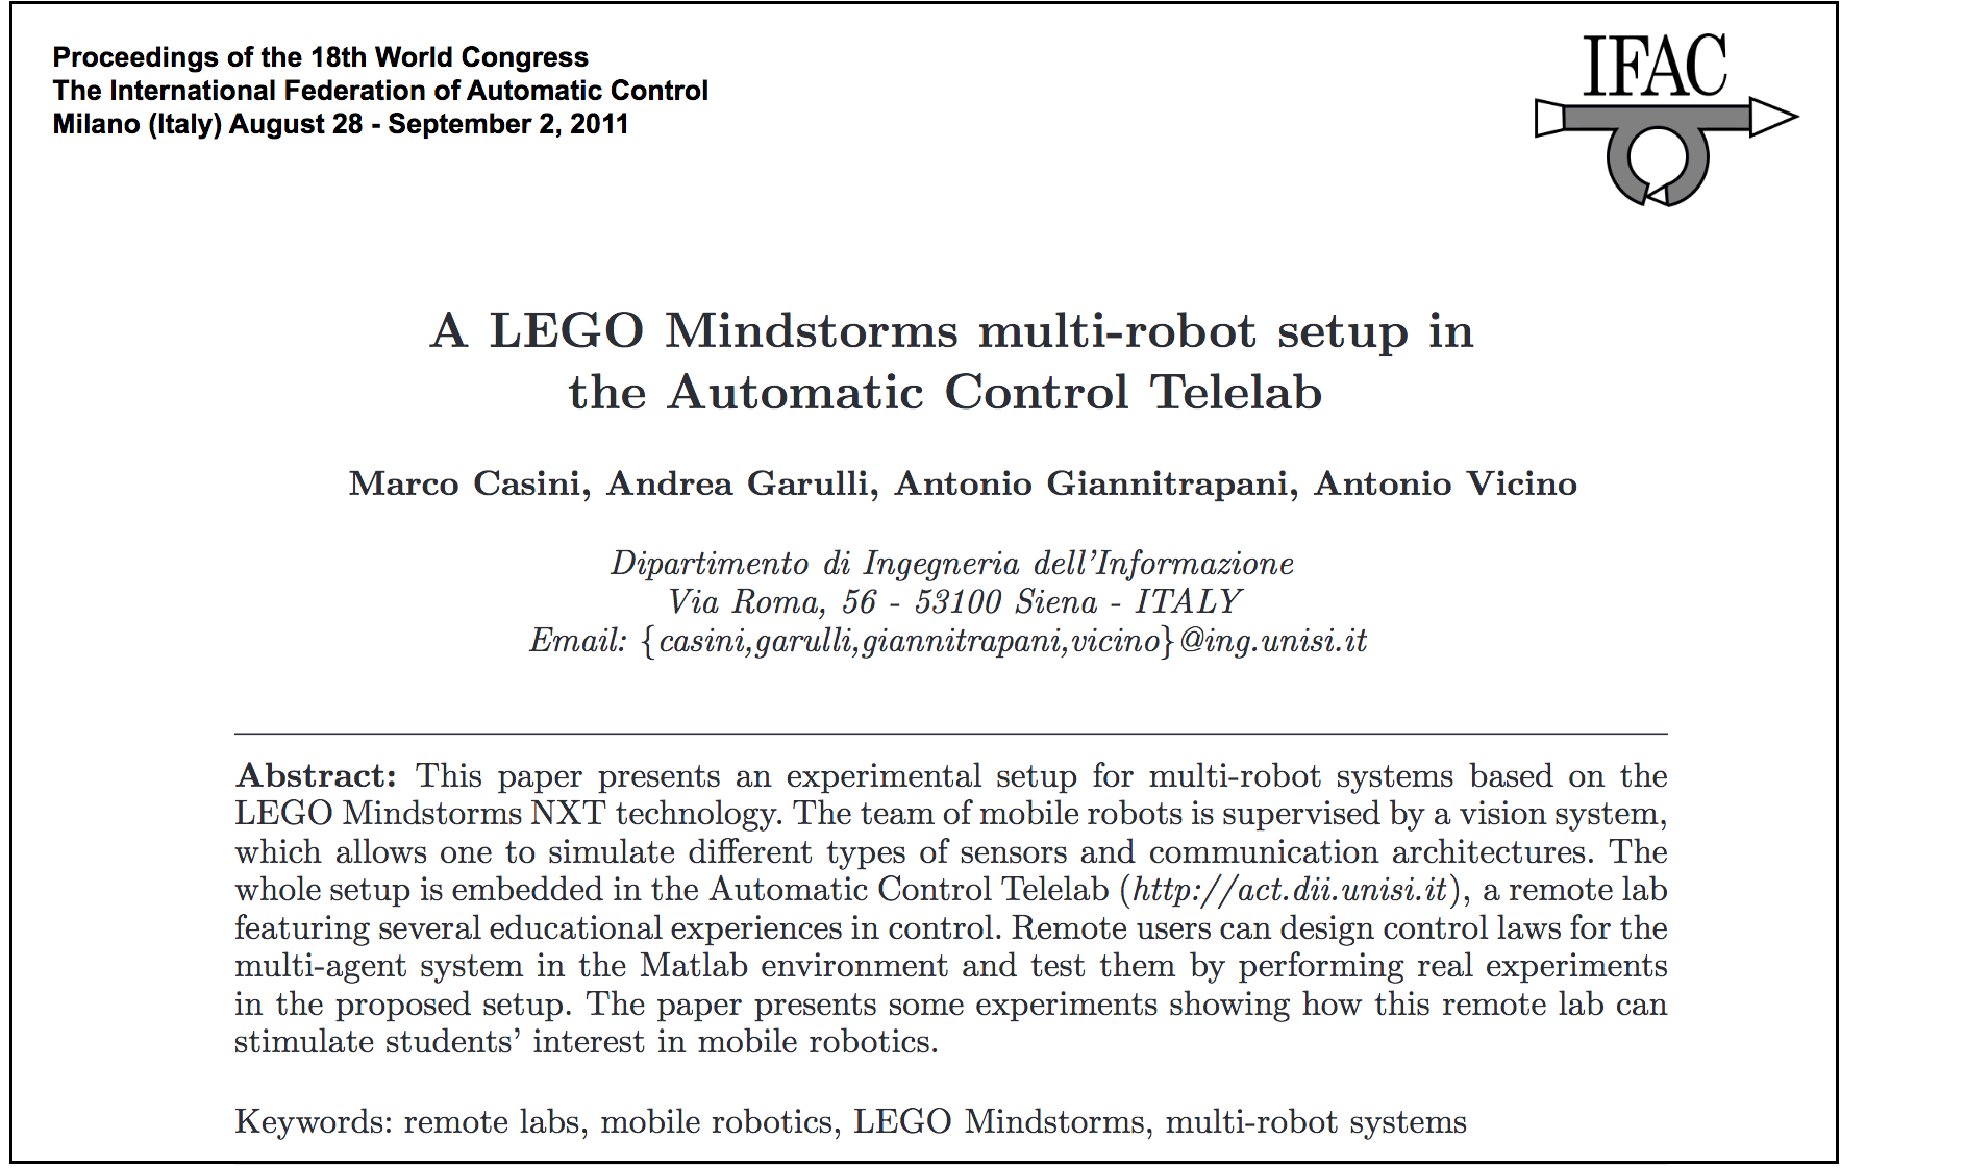
\includegraphics{proceedings}}
  \caption{Artikkel presentert ved konferanse.} 
  \label{fig:proceedings}
\end{figure}

\newpage

Siden denne artikkelen bare hadde 4 forfattere, 
får den {\em tag}'en  \fbox{\tt  CasGarGiaVic2011}
i .bib-fila, se under

\begin{boxedminipage}{160mm}
{\footnotesize{
\begin{verbatim}
@InProceedings{CasGarGiaVic2011,
  author = {Marco Casini and Andrea Garulli and Antonio Giannitrapani and Antonio Vicino},
  title = {A LEGO Mindstorms multi-robot setup in the Automatic Control Telelab},
  booktitle = {Proceedings of the 18th World Congress},
  year = {2011},
  pages = {9812--9817},
  organization = {IFAC},
}
\end{verbatim}
}}
\end{boxedminipage}

Den fullstendige beskrivelsen av {\tt InProceedings} er:

\begin{verbatim}
@InProceedings{,
  author = 	 {},
  title = 	 {},
  OPTcrossref =  {},
  OPTkey = 	 {},
  OPTbooktitle = {},
  OPTyear = 	 {},
  OPTeditor = 	 {},
  OPTvolume = 	 {},
  OPTnumber = 	 {},
  OPTseries = 	 {},
  OPTpages = 	 {},
  OPTmonth = 	 {},
  OPTaddress = 	 {},
  OPTorganization = {},
  OPTpublisher = {},
  OPTnote = 	 {},
  OPTannote = 	 {}
}
\end{verbatim}

\newpage

\subsection{\fbox{\tt @PhDThesis} og \fbox{\tt @MastersThesis}}
Dersom du skal referere til andre studenters
forskningsarbeid, kan du bruke 
{\tt @PhDThesis} og {\tt @MastersThesis}. Som du ser under nedenfor, 
benytter disse identiske elementer.
Det finnes også en 
{\tt @Thesis} som kan brukes for bacheloroppgaver.




\begin{verbatim}
@PhdThesis{,
  author = 	 {},
  title = 	 {},
  school = 	 {},
  year = 	 {},
  OPTkey = 	 {},
  OPTtype = 	 {},
  OPTaddress = 	 {},
  OPTmonth = 	 {},
  OPTnote = 	 {},
  OPTannote = 	 {}
}
\end{verbatim}

\begin{verbatim}
@MastersThesis{,
  author = 	 {},
  title = 	 {},
  school = 	 {},
  year = 	 {},
  OPTkey = 	 {},
  OPTtype = 	 {},
  OPTaddress = 	 {},
  OPTmonth = 	 {},
  OPTnote = 	 {},
  OPTannote = 	 {}
}
\end{verbatim}

\newpage
\section{Referering til litteratur, \fbox{\tt $\backslash$cite\{ \}}}
For å referere til de forskjellige litteraturelementene i 
\fbox{\tt referanser.bib}, må du bruke \fbox{\tt
  $\backslash$cite}-kommandoen som vist i følgende eksempel.

\begin{boxedminipage}{\textwidth}
\begin{verbatim}
Som vist i~\cite{Dre2019} kan numerisk integrasjon benyttes til ...
\end{verbatim}
\end{boxedminipage}

og denne vil fremstå slik:

Som vist i~\cite{Dre2019} kan numerisk integrasjon benyttes til ...


Det er vanlig at referanselisten kommer etter konklusjonen.
For å få dette til må du inkludere følgende
kodelinjer i hovedfilen rett etter konklusjonskapittelet:

\begin{boxedminipage}{\textwidth}
\begin{verbatim}
\bibliographystyle{plain}
\bibliography{referanser.bib}
\addcontentsline{toc}{chapter}{Bibliografi} 
\end{verbatim}
\end{boxedminipage}

Første linje forteller hvilken stil du ønsker å bruke. 
Stilen som heter \fbox{\tt plain} plasserer et tall foran hver
referanse i referanselista, og det er dette tallet som vises i
teksten. 

Andre linje forteller {\LaTeX} hvilken .bib-fila som skal
benyttes. Her kan det stå flere filnavn.

Siste linje legger til ``Bibliografi''-kapittelet i innholdsfortegnelsen.


